\section{Durchführung}
\label{sec:Durchführung}
Vor den Messungen werden für diesen Veruch drei periodische Funktionen gewählt und in eine Fourierreihen nach Gleichung \eqref{eq:gl1} entwickelt.
\subsection{Fourier-Transformation}
Diese Funktionen werden dann mit einem mit einem Funktionsgenerator erstellt und auf einem digitalen Oszilloskop ausgelesen.
Der Grundaufbau für diesen Versuch ist in Abbildung \ref{fig:aufbau} dargestellt.
\begin{figure}[H]
    \centering
    \caption{Versuchsaufbau für die Transformation eines Signals.}%\cite{v351}}
    \label{fig:aufbau}
    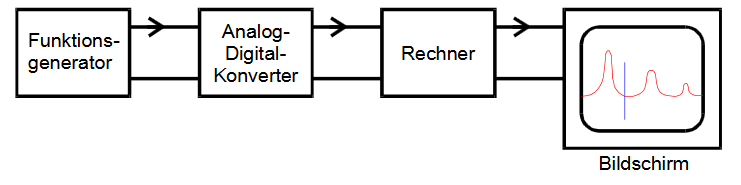
\includegraphics[width=\textwidth-20em]{content/aufbau.png}
\end{figure}
\noindent
Das Oszilloskop transformiert das eingehende Signal und wirft das Frequenzspektrum auf den Bildschirm.
Da über einen endlichen Zeitraum integriert wird ist das Linienspektrum unschärfer als Abbildung \ref{fig:lspek} darstellt.
Die Koeffizienten sind nicht als $\delta$-Distributionen zu erwarten, sondern als Linien endlicher breite.
Für die drei entwickelten Funktionen werden mit einem "Cursor" die ersten neun nicht verschwindenen Koeffizienten gemessen.
\subsection{Fourier-Synthese}
